\chapter{Sprint 1: User Management}

\section{Introduction}
In this chapter we will discuss the user management side of our project.
We focused on implementing the authentication and authorization
flow for our system users and how we can manage them in our system.

We Have Three Types of Users That we should manage and allow them to use the platform
each with a given access level to assure its security and confidentiality. The three users are:

Admin: Which is basically responsible for the creation of the ODC coordinators accounts
and other features that are illustrated in the use case diagram bellow.

ODC Coordinator: Which is responsible for the creation of the ODC experts accounts, and managing events

ODC Expert: Which is responsible for the technical part of the system, such as creating and managing problems,
add quizzes and so on.

to achieve this separation of concerns and to assure the security of the system we used a token-based authentication.
we chose the security standard JWT (JSON Web Token) to implement the authentication, and a role based access control
to manage the access level of each user. Adding to that we used the bcrypt library to hash passwords and store them securely.

\section{Sprint backlog}
Before we start implementing the user management module, we defined the tasks needed in the sprint backlog.
to share the same vision and share responsibilities between the team members. The following table shows the tasks
we defined for the user management module.

\begin{longtable}{|>{\raggedright\arraybackslash}p{2cm}|>{\raggedright\arraybackslash}p{3cm}|>{\raggedright\arraybackslash}p{8cm}|}
  \caption{User Management Module Features}                                                                     \\
  \hline
  \textbf{ID} & \textbf{Functionality}      & \textbf{Feature}                                                  \\ \hline
  \endhead

  \hline
  \endfoot

  \hline
  \endlastfoot

  1           & \textbf{Authentication}     & 1.1 As an ODC admin, I can authenticate                           \\ \cline{3-3}
              &                             & 1.2 As an ODC coordinator, I can authenticate                     \\ \cline{3-3}
              &                             & 1.3 As an ODC expert, I can authenticate                          \\ \hline
  2           & \textbf{User Management}    & 2.1 As an ODC admin, I can add an ODC coordinator                 \\ \cline{3-3}
              &                             & 2.2 As an ODC admin, I can list all ODC coordinators accounts     \\ \cline{3-3}
              &                             & 2.3 As an ODC admin, I can list all ODC experts accounts          \\ \cline{3-3}
              &                             & 2.4 As an ODC admin, I can search all ODC coordinators accounts   \\ \cline{3-3}
              &                             & 2.5 As an ODC coordinator, I can list all ODC experts accounts    \\ \cline{3-3}
              &                             & 2.6 As an ODC coordinator, I can add an ODC expert account        \\ \cline{3-3}
              &                             & 2.7 As an ODC coordinator, I can list all ODC experts accounts    \\ \cline{3-3}
              &                             & 2.8 As an ODC coordinator, I can search ODC experts accounts list \\ \cline{3-3}
              &                             & 2.9 As an ODC coordinator, I can disable an expert account        \\ \hline
  3           & \textbf{Profile Management} & 3.1 As an ODC admin, I can update my profile                      \\ \cline{3-3}
              &                             & 3.2 As an ODC admin, I can change my password                     \\ \cline{3-3}
              &                             & 3.3 As an ODC coordinator, I can update my profile                \\ \cline{3-3}
              &                             & 3.4 As an ODC coordinator, I can change my password               \\ \cline{3-3}
              &                             & 3.5 As an ODC expert, I can update my profile                     \\ \cline{3-3}
              &                             & 3.6 As an ODC expert, I can change my password                    \\ \hline
\end{longtable}

\newpage
\section{Uml And Design}
We used the following UML diagram to design the user management module.

\begin{figure}[h!]
  \centering
  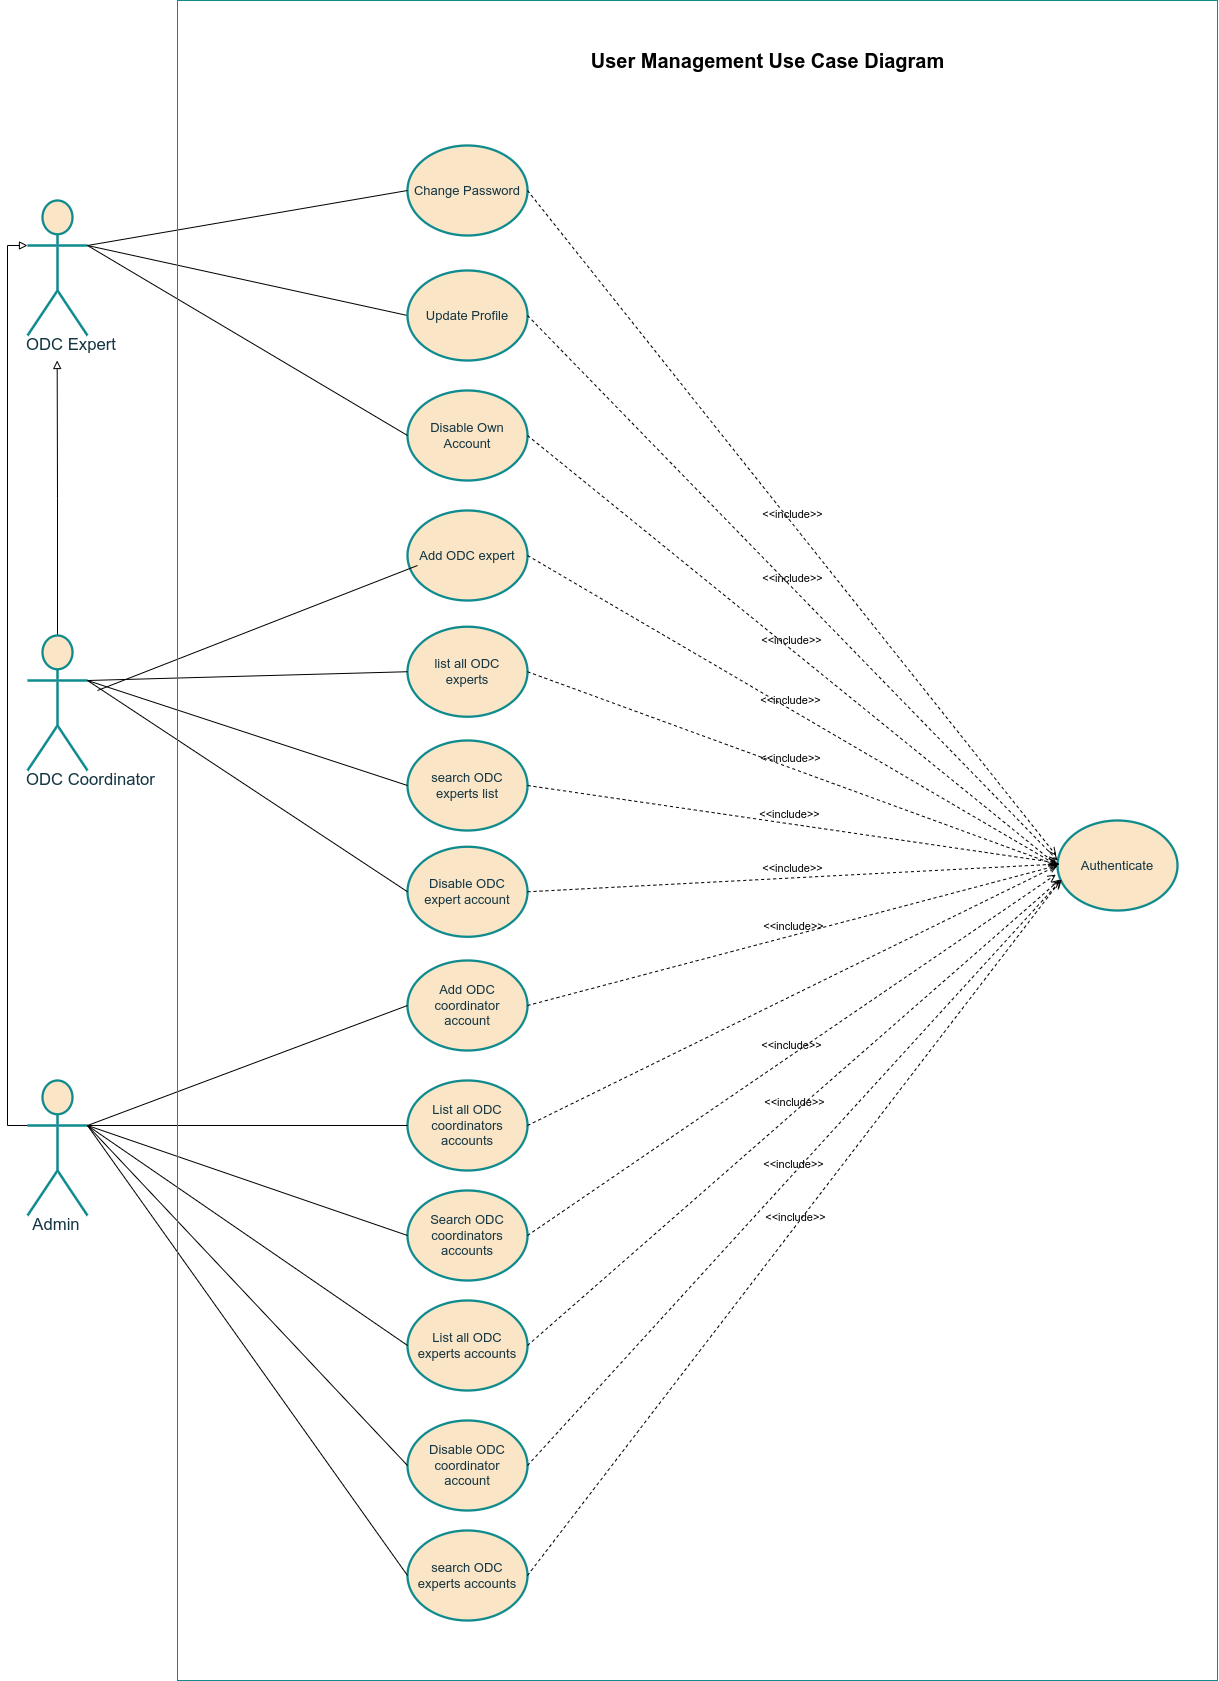
\includegraphics[width=0.8\textwidth]{images/userManagementUseCase.drawio.png}
  \caption{User Management UML Diagram}
\end{figure}

Now for the design of the user management module, we used the following MongoDB schema to store the user data.

\begin{figure}[htp!]
  \centering
  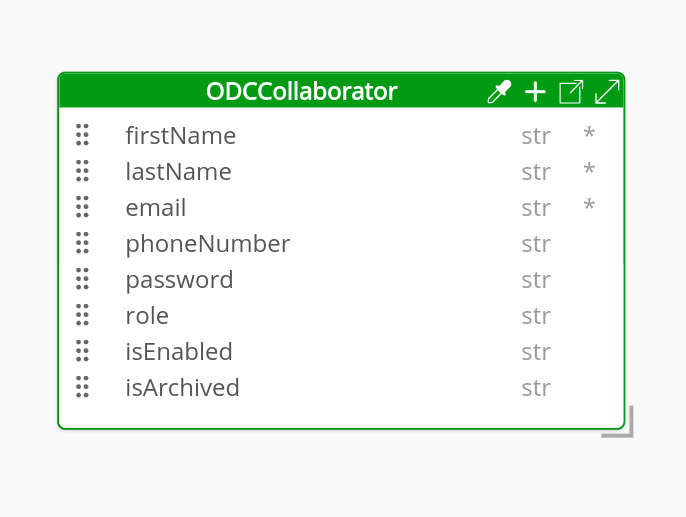
\includegraphics[width=0.8\textwidth]{images/diagram-ODCCollaborator.png}
  \caption{User Management Schema}
\end{figure}

The following figure represents the use case diagram for our first sprint.

\subsection{Textual Description of the login feature}

\begin{table}[h!]
  \centering
  \begin{tabular}{|c|c|}
    \hline
    Use Case           & authenticate                                                                                                                           \\
    \hline
    Actor              & \begin{tabular}[c]{@{}l@{}} User: Collaborator/Administrator
                         \end{tabular}                                                                            \\
    \hline
    Brief Description  & \begin{tabular}[c]{@{}l@{}} The user must be registered in the database and must know their credentials
                         \end{tabular}                                 \\
    \hline
    Pre-condition      & \begin{tabular}[c]{@{}l@{}} The user must have their access parameters
                         \end{tabular}                                                                  \\
    \hline
    Post-condition     & \begin{tabular}[c]{@{}l@{}} The user is successfully authenticated
                         \end{tabular}                                                                      \\
    \hline
    Main Scenario      & \begin{tabular}[c]{@{}l@{}} 1. The user enters their credentials (email and password) in the appropriate fields \\and submits the form.
                           \\ 2. The system verifies the information entered by the user
                           \\3. The system displays the appropriate interface according to the role of the user
                         \end{tabular} \\
    \hline
    Exception Scenario & \begin{tabular}[c]{@{}l@{}} 1.1 The entered data is incorrect or missing:
                           \\  2.1.1 The system displays an error message and the use case returns to step 1 of the main scenario
                           \\2.1 The entered credentials do not exist in the database:
                           \\2.1.1 The system displays an error message and the use case returns to step 2 of the main scenario
                         \end{tabular}                                  \\
    \hline
    Extension          & \begin{tabular}[c]{@{}l@{}} In case of forgotten password, the user can redefine a new password
                         \end{tabular}                                         \\
    \hline
  \end{tabular}

  \begin{center}
    \caption{Backlog for the First Sprint}
    \label{tab:Backlog for the First Sprint}
  \end{center}
\end{table}

\subsection{the sequence diagram of the login feature}

\begin{figure}[h!]
  \centering
  "The following figure represents the sequence diagram for the use case 'authenticate'."\\
  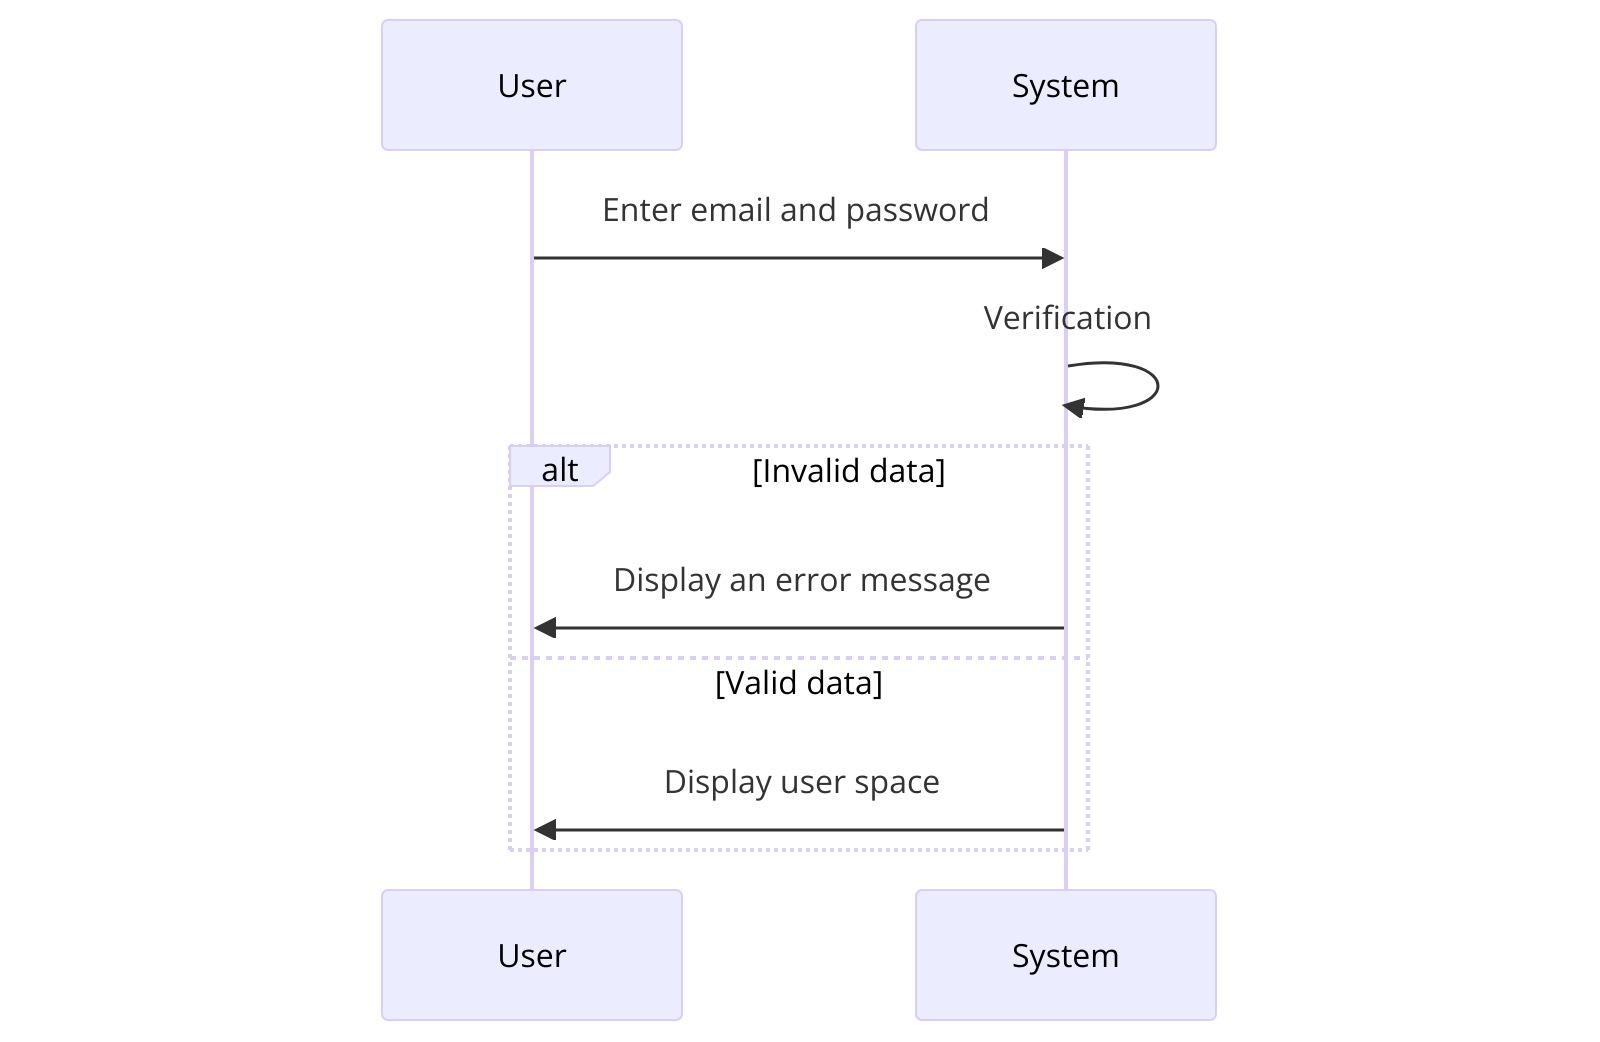
\includegraphics[width=0.8\textwidth]{images/diagram seq.png}
  \caption{the sequence diagram for the use case 'authenticate'}
  \label{fig:the sequence diagram for the use case 'authenticate'}
\end{figure}

\section{User Interfaces}

The following figures show the user interfaces of the user management module after implementing
the functionalities that are defined in the sprint backlog.

\begin{figure}[h!]
  \centering
  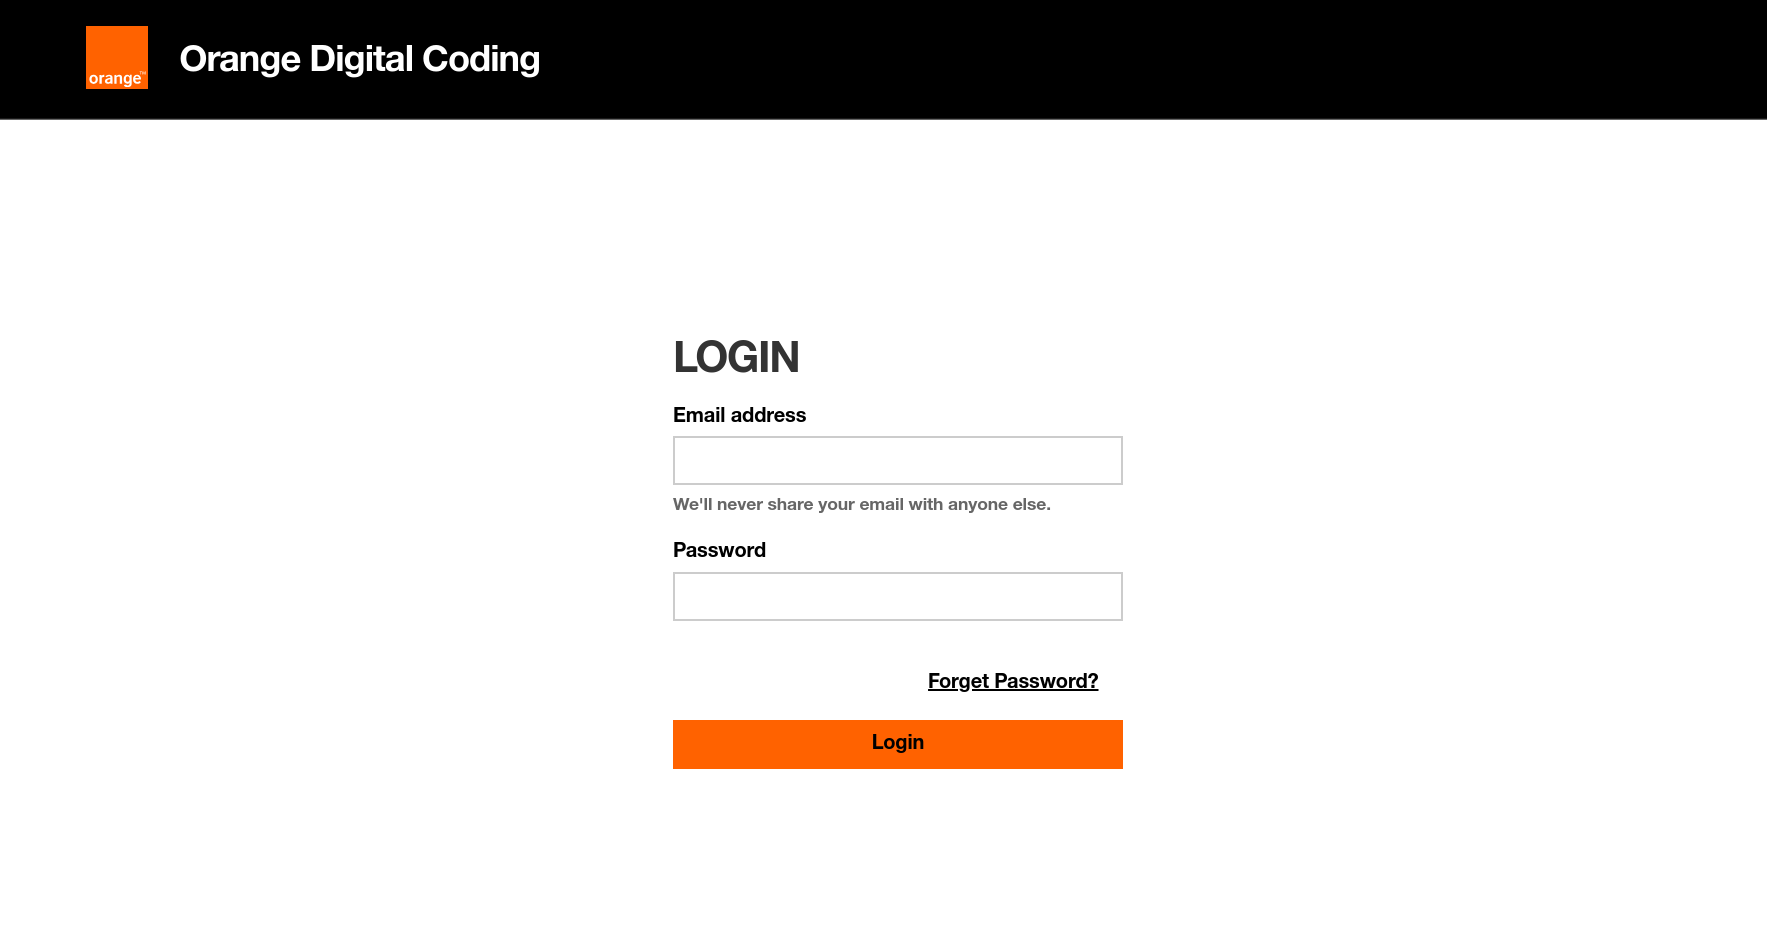
\includegraphics[width=0.8\textwidth, height=0.3\textheight]{images/odc-login.png}
  \caption{Login Page}
\end{figure}

\begin{figure}[h!]
  \centering
  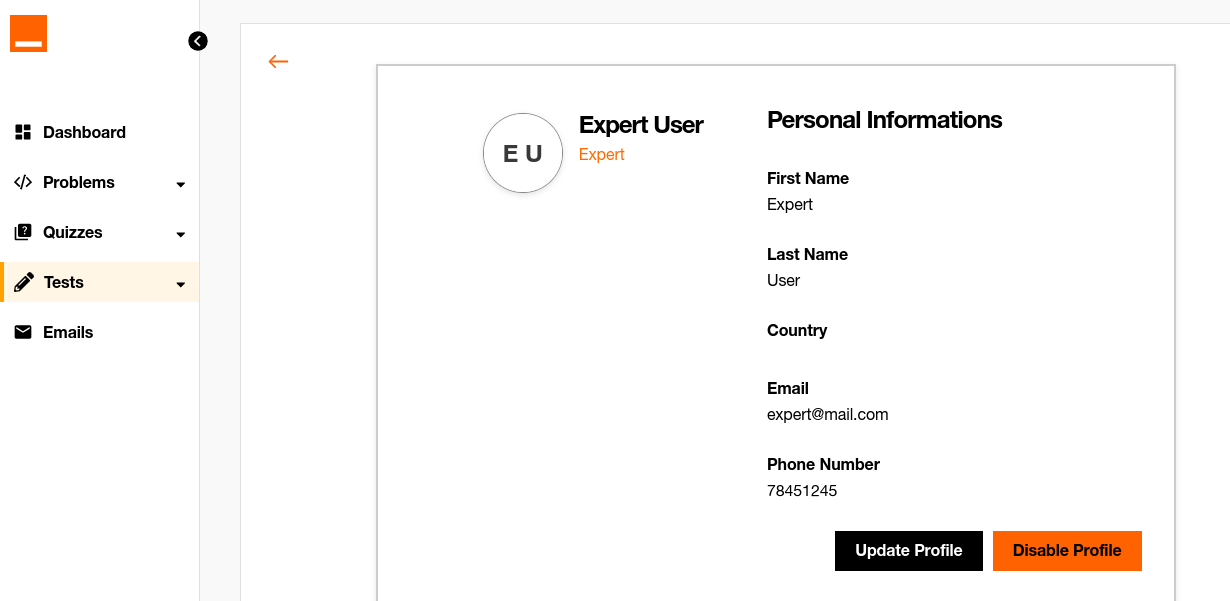
\includegraphics[width=0.8\textwidth, height=0.3\textheight]{images/odc-view-profile.png}
  \caption{View Profile}
\end{figure}


\begin{figure}[h!]
  \centering
  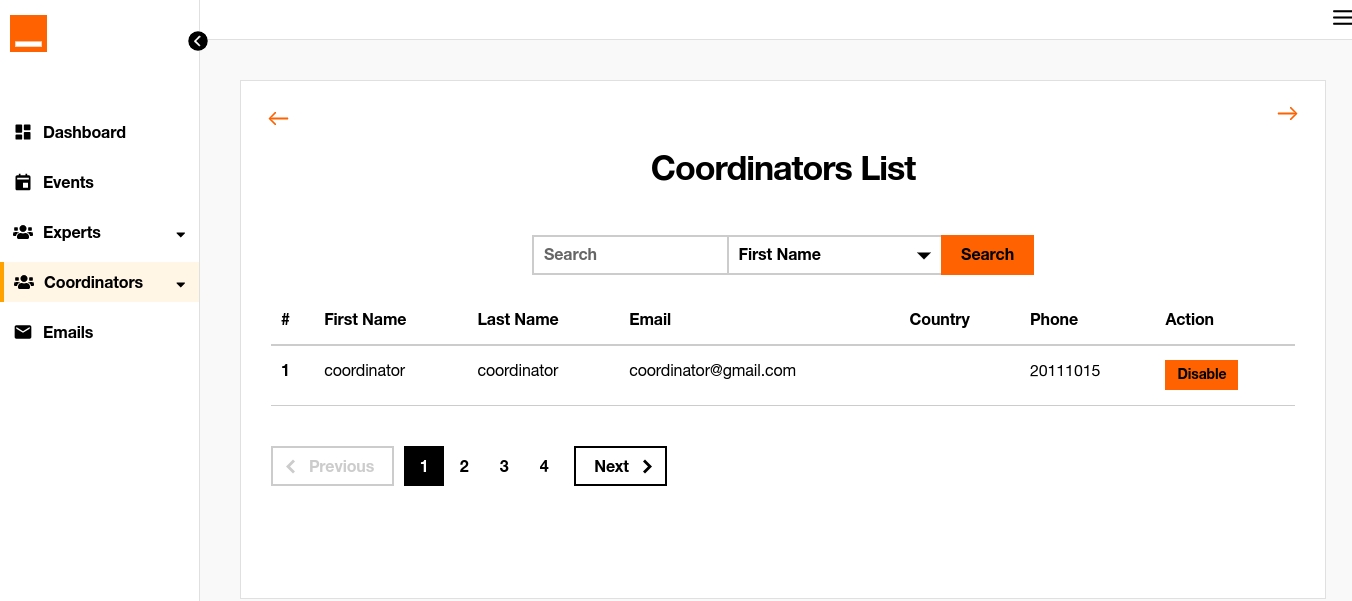
\includegraphics[width=0.8\textwidth, height=0.3\textheight]{images/odc-coordinators-list.png}
  \caption{ODC coordinators list}
\end{figure}


\begin{figure}[h!]
  \centering
  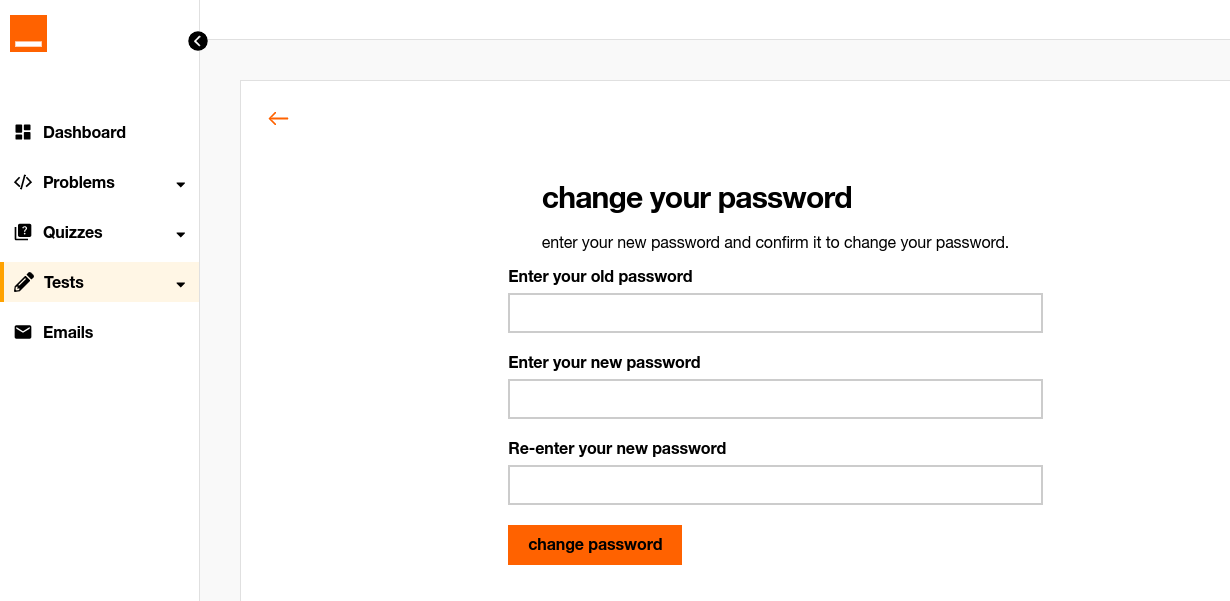
\includegraphics[width=0.8\textwidth, height=0.3\textheight]{images/odc-change-password.png}
  \caption{Change Password}
\end{figure}

\begin{figure}[h!]
  \centering
  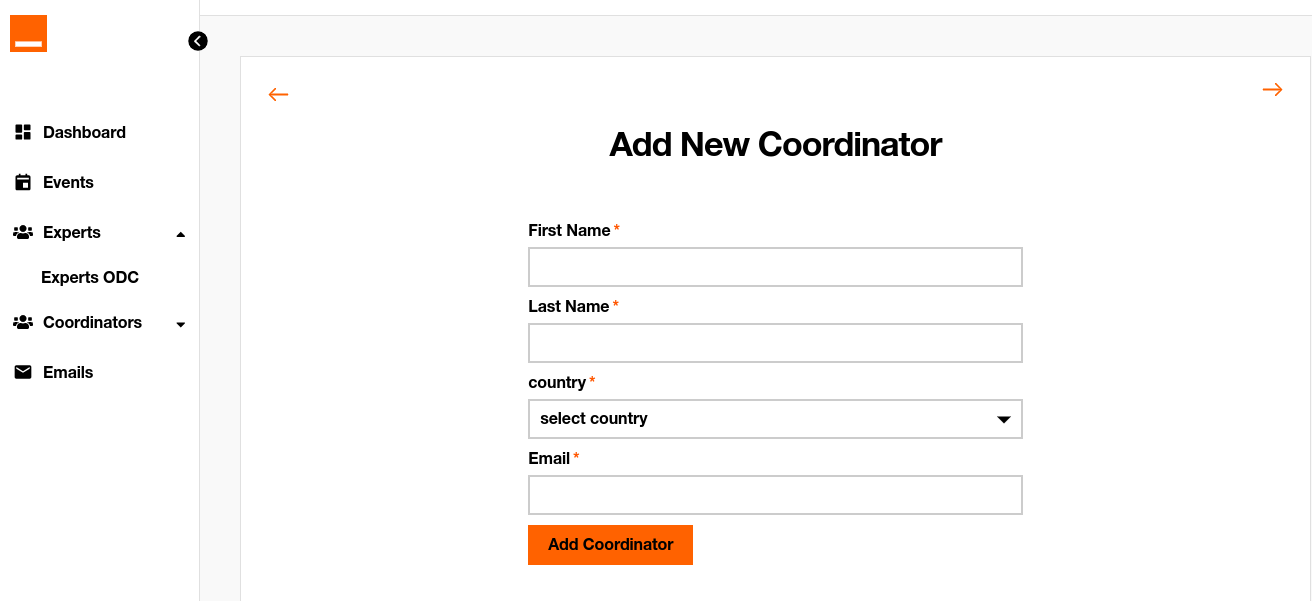
\includegraphics[width=0.8\textwidth, height=0.3\textheight]{images/odc-add-new-coordinator.png}
  \caption{Add New Coordinator}
\end{figure}
